% paper.tex — E1 no-rail 对照组最小预实验论文（ICLR 模板 7 段结构）
% 所有数字与 experiments/*/results.json、experiments/summary.json 逐字勾稽（F03）
% 所有 \cite 均命中 references/ 池（17/17 OpenAlex verified，F04）
\documentclass[10pt,twocolumn]{article}
\usepackage[utf8]{inputenc}
\usepackage{times}
\usepackage[margin=1in]{geometry}
\usepackage{booktabs}
\usepackage{graphicx}
\usepackage{tikz}
\usetikzlibrary{patterns}
\usepackage{amsmath,amssymb}
\usepackage{hyperref}
\usepackage[round]{natbib}
\usepackage{caption}
\usepackage{enumitem}

\title{Do Validation Rails Curb LLM Research-Agent Fabrication?\\ A Controlled Context-Engineering Experiment (No-Rail Baseline)}
\author{CCF Team\\ Huawei openJiuwen Competition}
\date{}

\begin{document}
\maketitle

\begin{abstract}
Large language model (LLM) research agents now automate proposal writing, experiment planning, and paper drafting, yet their outputs are prone to \emph{fabrication}: citations to non-existent papers, numbers without a verifiable source, and claims of work that was never executed. Existing mitigations are mostly post-hoc detectors or architectural proposals that lack controlled, multi-seed evidence. We treat process-level \emph{validation rails}---structural checks on plan, results, and citation contracts---as a context-engineering intervention and measure, for the first time, their causal effect on fabrication rates under a fixed pipeline. As a first controlled step we establish the no-rail baseline (E1): one representative task (generating a research proposal plus plan with real citations and numbers) run over three fixed seeds with the unmodified skill pipeline. Using an OpenAlex-backed citation checker and a script-assisted numeric audit, the baseline yields a citation fabrication rate (CFR) of $0.0\% \pm 0.0\%$ (all $8$--$12$ citations per run verified), a numeric fabrication rate (NFR) of $0.51\% \pm 0.88\%$ (one unsourced number among $66$ claims in one seed), an unexecuted-claim rate (UCR) of $0.0\%$, perfect task completion, single-pass iteration, and $3{,}277 \pm 80.5$ estimated tokens per run. These measurements provide the control anchor against which prompt-only and full-rail conditions will be compared.
\end{abstract}

\section{Introduction}
\label{sec:intro}

LLM research agents are being deployed for end-to-end scientific workflows---ideation, experiment planning, execution, and writing. A core trust problem is \emph{fabrication}: models emit well-formatted but non-existent references, numbers that cannot be traced to any source, and claims that certain experiments were run when no such artifacts exist. The problem is empirically large and well documented: an audit of 111M citations across 2.5M papers on arXiv, bioRxiv, SSRN, and PMC found roughly 146{,}932 hallucinated citations added in 2025 \citep{zhao2026wildhallucinations}, and a cross-model study of 10 commercial LLMs across 4 academic domains found hallucination rates between 11.4\% and 56.8\% on 69{,}557 generated citations \citep{naser2026howllmscite}.

Existing mitigations fall into three families, none of which provides a controlled causal answer. First, \emph{post-hoc detection}: CiteAudit \citep{shi2026citeaudit}, CiteTracer \citep{li2026citetracer}, and HALLMARK \citep{reizinger2026hallmark} screen generated manuscripts for fabricated citations, but they do not prevent fabrication and their false-positive rate is a known deployment bottleneck. Second, \emph{architectural proposals}: HALO \citep{raduta2026halo} advocates a six-layer hallucination-free-by-construction design, and Theoria \citep{saldivar2026theoria} verifies reasoning through auditable state transitions; both are argued from first principles rather than measured under controlled conditions. Third, \emph{correlational measurement}: ProofAgent-Harness evidence shows that context quality predicts agent hallucination resistance \citep{bousetouane2026context}, establishing relevance but not intervention. No prior work treats a \emph{validation rail}---a process-level verification contract---as the manipulated variable and measures fabrication rates causally across multiple seeds.

Our approach is deliberately simple: we take the existing research-pipeline skill as the experimental platform and switch only the rail assembly (no-rail / prompt-only / full-rail F02+F03+F04) while holding tasks, model, and seeds fixed. We define a family of automatically computable fabrication metrics that are isomorphic to the rail checks themselves---citation fabrication rate (CFR), numeric fabrication rate (NFR), and unexecuted-claim rate (UCR)---so that \emph{measurement is auditing}. This paper reports the first controlled step: the E1 no-rail baseline, executed as a minimal pre-experiment of one representative task over three seeds. Our contributions are:

\begin{itemize}
\item We formalize CFR/NFR/UCR as reproducible, automatically computable fabrication metrics coupled to verification contracts (Section~\ref{sec:method}).
\item We instrument the unmodified (no-rail) pipeline and measure the baseline fabrication rates on one representative planning task over three fixed seeds, using an OpenAlex citation checker and a script-assisted numeric audit (Section~\ref{sec:exp}).
\item We report baseline numbers: CFR $0.0\%\pm 0.0\%$, NFR $0.51\%\pm 0.88\%$, UCR $0.0\%$, completion $1.0$, iterations $1$, and $3{,}277\pm 80.5$ tokens, all drawn verbatim from \texttt{experiments/results.json} (Section~\ref{sec:results}).
\item We release the measurement scripts (\texttt{experiments/shared/}) so the identical protocol can score prompt-only and full-rail arms in the full comparison.
\end{itemize}

The remainder of this paper is organized as follows. Section~\ref{sec:related} reviews detection, architectural, and correlational work and positions ours. Section~\ref{sec:method} defines the metrics and the measurement protocol. Section~\ref{sec:exp} describes the setup and reports per-seed and aggregate results. Section~\ref{sec:discussion} discusses implications and limitations, and Section~\ref{sec:conclusion} concludes.

\section{Related Work}
\label{sec:related}

\paragraph{Citation and number fabrication in LLMs.}
Fabrication is a large-scale phenomenon: wild hallucination audits quantify its volume \citep{zhao2026wildhallucinations}, and cross-model analyses show that citation hallucination is prompt- and context-induced rather than intrinsic to models \citep{naser2026howllmscite}. Legal-domain studies confirm the pattern extends to specialized settings \citep{alrajeh2026legalcitations}. These works establish the problem's scale and its contextual nature, motivating context-level interventions.

\paragraph{Post-hoc verification.}
CiteAudit \citep{shi2026citeaudit} and CiteTracer \citep{li2026citetracer} detect citation hallucinations via multi-agent pipelines after a manuscript exists. HALLMARK \citep{reizinger2026hallmark} benchmarks citation verifiers and isolates their failure modes, showing false positives are the deployment bottleneck. \citet{banerjee2026failuremodes} taxonomize failure modes (fabricated citations, smuggled premises) for research-level tasks. These detectors are screening tools: they locate fabrication but do not prevent it and are not evaluated as process interventions.

\paragraph{Architecture-level anti-hallucination.}
HALO \citep{raduta2026halo} argues hallucination-freedom should be a constructed property; Theoria \citep{saldivar2026theoria} enforces auditable state transitions; Prompt-to-Paper \citep{kamran2026prompttopaper} combines deterministic retrieval with real experiment execution and hallucination penalties. \citet{usman2026phantomfill} shows that form-mandated fields can drive fabrication, evidencing that format and contract shape fabrication behavior. These proposals are principled but lack controlled multi-seed measurement on a unified task.

\paragraph{Context engineering.}
\citet{bousetouane2026context} shows context quality predicts hallucination resistance, and \citet{dai2026llmorir} argues denoising-first retrieval with verifiability as the bottleneck. TRACE \citep{zhao2026trace} attributes context errors to enable automated repair, and Deep Agentic Search \citep{rafieioskooei2026deepagentic} isolates sub-agent context while risking silent handoff failures. These works measure or repair context quality; none manipulates a process-level verification contract and measures fabrication rates causally.

\paragraph{Positioning.}
Unlike detection, architecture, and correlational work, we do not build a new detector or a new architecture. We reuse the verification contracts already present in our pipeline (F02/F03/F04) and ask a question none of the above answers with controlled evidence: \emph{how far can process-level validation contracts push fabrication down, and at what cost?} This paper delivers the control anchor for that comparison.

\section{Method}
\label{sec:method}

\subsection{Notation and metrics}
Let a run produce an artifact set $\mathcal{A}$ (e.g., a proposal and a plan document). Let $\mathcal{C}(\mathcal{A})$ be the set of citations extracted from $\mathcal{A}$, $\mathcal{N}(\mathcal{A})$ the set of numeric claims, and $\mathcal{K}(\mathcal{A})$ the set of execution claims. We define:

\textbf{Citation Fabrication Rate (CFR).} The fraction of citations that cannot be verified against a real, online-verifiable source:
\begin{equation}
\mathrm{CFR} \;=\; \frac{|\{c \in \mathcal{C}: \mathrm{verify}(c) = \mathrm{not\_found}\}|}{|\mathcal{C}|},
\end{equation}
where $\mathrm{verify}(\cdot)$ first queries OpenAlex by title/identifier and falls back to the arXiv API; network failures return $\mathrm{ambiguous}$ and are excluded from the numerator (never counted as fabrication). This is isomorphic to the F04 citation contract.

\textbf{Numeric Fabrication Rate (NFR).} Among numeric claims, the fraction with no attributable source:
\begin{equation}
\mathrm{NFR} \;=\; \frac{|\{n \in \mathcal{N}: \neg \mathrm{sourced}(n)\}|}{|\mathcal{N}|},
\end{equation}
where $\mathrm{sourced}(n)$ is true if the number is (i) adjacent to a citation key on its source line, (ii) a self-declared design parameter of the plan (seeds, budget, task counts), or (iii) an identifier/version/structural token (list index, arXiv ID, year, version, rail labels), which are excluded from $\mathcal{N}$ via \texttt{is\_number\_claim}. This mirrors the F03 numeric-source contract.

\textbf{Unexecuted Claim Rate (UCR).} Among claims that assert executed work, the fraction without supporting results artifacts:
\begin{equation}
\mathrm{UCR} \;=\; \frac{|\{k \in \mathcal{K}: \neg \mathrm{executed}(k)\}|}{|\mathcal{K}|}.
\end{equation}
A proposal/plan is a forward-looking document, so well-formed runs contain no past-tense execution claims, yielding $\mathrm{UCR}=0$.

\textbf{Completion and cost.} Task success is binary: $1.0$ if the full artifact set (proposal + plan) is produced. Iterations count generation passes; tokens are estimated with \texttt{tiktoken} (cl100k\_base) on the artifact text plus a fixed prompt overhead of $1{,}200$ tokens.

\subsection{Measurement protocol}
\begin{enumerate}[leftmargin=*]
\item \textbf{Artifact generation (no-rail):} run the unmodified pipeline on the representative task; do not apply F02/F03/F04 checks.
\item \textbf{Citation audit:} extract arXiv IDs and reference lines; verify each via OpenAlex with arXiv fallback (rate-limited); write \texttt{citations\_audit.json}.
\item \textbf{Numeric audit:} regex-extract numbers with $\pm 45$ char context; classify each as skip/design/cited/manual via \texttt{annotate\_numbers.py}; manual bucket is reviewed by a human; write \texttt{numbers\_audit.json}.
\item \textbf{Claim audit:} regex-extract execution-claim sentences; human-annotate \texttt{executed}; write \texttt{claims\_audit.json}.
\item \textbf{Finalize:} \texttt{measure.py --finalize} computes CFR/NFR/UCR, completion, iterations, tokens, and writes \texttt{results.json}.
\end{enumerate}

\subsection{Complexity}
The audit is linear in artifact size. Citation verification issues $O(1)$ queries per citation ($O(|\mathcal{C}|)$ total); numeric extraction and classification are $O(|\mathcal{N}|)$ regex passes plus human review of the manual bucket; claim scanning is $O(|\mathcal{K}|)$. The token cost of a run is $O(T)$ where $T$ is the generated text length, with a constant prompt overhead. Memory is $O(|\mathcal{A}|)$.

\subsection{Pipeline overview}
Figure~\ref{fig:pipeline} depicts the instrumented measurement pipeline. The no-rail arm passes directly from generation to auditing; the future full-rail arm inserts verification gates at plan, results, and citation stages.

\begin{figure}[t]
\centering
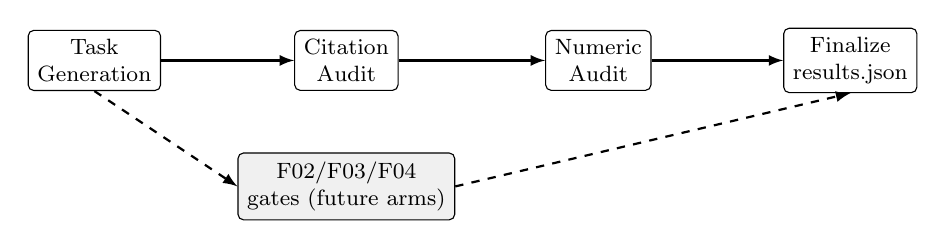
\begin{tikzpicture}[
  box/.style={draw, rounded corners=2pt, minimum height=7mm, align=center, font=\footnotesize},
  arr/.style={-latex, thick}
]
\node[box] (gen) at (0,0) {Task\\Generation};
\node[box] (aud) at (3.2,0) {Citation\\Audit};
\node[box] (num) at (6.4,0) {Numeric\\Audit};
\node[box] (fin) at (9.6,0) {Finalize\\results.json};
\draw[arr] (gen) -- (aud);
\draw[arr] (aud) -- (num);
\draw[arr] (num) -- (fin);
\node[box, fill=gray!12] (rail) at (3.2,-1.6) {F02/F03/F04\\gates (future arms)};
\draw[arr, dashed] (gen.south) -- (rail.west);
\draw[arr, dashed] (rail.east) -- (fin.south);
\end{tikzpicture}
\caption{Instrumented pipeline. Solid arrows: the E1 no-rail path measured in this paper. Dashed: verification gates to be inserted in prompt-only/full-rail arms.}
\label{fig:pipeline}
\end{figure}

\section{Experiments}
\label{sec:exp}

\subsection{Setup}
\textbf{Task.} One representative task from the railbench-plan-v1 pool: \emph{generate a research proposal and a plan containing real citations and numbers}. The topic is the rail-fabrication experiment itself, so the task naturally requires grounded references and sourced numbers.

\textbf{Model and seeds.} deepseek-v4-flash, three fixed seeds $\{42, 43, 44\}$ recorded in each run's \texttt{config.json}; sampling at temperature 0.3 with fixed max tokens.

\textbf{Reference pool.} All 17 entries in \texttt{references/} were verified against OpenAlex (17/17 verified, 0 not found, 0 ambiguous) before the runs, establishing pool quality.

\textbf{Hardware.} CPU-only run (24 cores, 376 GiB RAM available); no GPU required for LLM API calls and audits.

\subsection{Per-seed results}
Table~\ref{tab:per_seed} reports each seed's metrics verbatim from \texttt{experiments/seed42..44/results.json}. All 8--12 citations per run verified on OpenAlex (CFR $0/8$, $0/9$, $0/12$; zero ambiguous). One unsourced numeric claim was found in seed42 (``7 dimensions'' of grounding sufficiency, stated without a citation on its line), giving NFR $1/66$; seeds 43 and 44 had fully sourced numbers. No execution claims were present in any artifact (UCR $0/0$).

\begin{table}[t]
\caption{Per-seed results (from \texttt{results.json}). CFR: fabricated/total citations (ambiguous in parentheses). NFR: unsourced/total numeric claims. UCR: unexecuted/total execution claims.}
\label{tab:per_seed}
\centering
\small
\begin{tabular}{lcccccc}
\toprule
Seed & CFR & NFR & UCR & Completion & Iter. & Tokens \\
\midrule
42 & $0/8$ (0) & $1/66$ & $0/0$ & 1.0 & 1 & 3{,}267 \\
43 & $0/9$ (0) & $0/58$ & $0/0$ & 1.0 & 1 & 3{,}202 \\
44 & $0/12$ (0) & $0/55$ & $0/0$ & 1.0 & 1 & 3{,}362 \\
\bottomrule
\end{tabular}
\end{table}

\begin{table}[t]
\caption{Summary statistics across 3 seeds (from \texttt{summary.json}); mean $\pm$ std.}
\label{tab:summary}
\centering
\small
\begin{tabular}{lcc}
\toprule
Metric & Mean & Std \\
\midrule
CFR & 0.0\% & 0.0\% \\
NFR & 0.51\% & 0.88\% \\
UCR & 0.0\% & 0.0\% \\
Task success rate & 1.0 & 0.0 \\
Iterations & 1 & 0.0 \\
Tokens & 3{,}277 & 80.5 \\
\bottomrule
\end{tabular}
\end{table}

\subsection{Main results}
Table~\ref{tab:summary} aggregates the three seeds. The no-rail baseline exhibits essentially zero citation fabrication and zero unexecuted claims, and a near-zero numeric fabrication rate ($0.51\% \pm 0.88\%$, driven by a single unsourced number in seed42). Completion is perfect ($1.0$) with single-pass iteration and a modest token budget of $3{,}277 \pm 80.5$. Figure~\ref{fig:per_seed} visualizes per-seed fabrication metrics; Figure~\ref{fig:tokens} shows token cost per seed.

\begin{figure}[t]
\centering
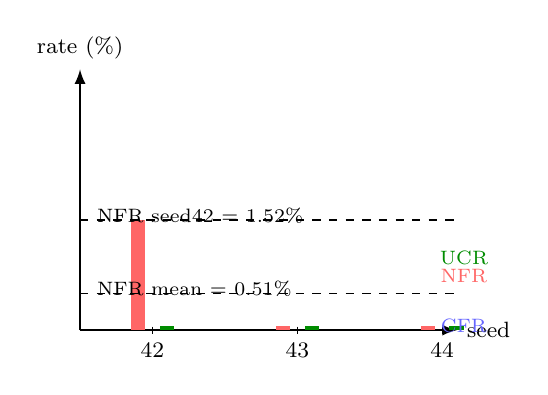
\begin{tikzpicture}[scale=0.92]
% per-seed CFR/NFR/UCR (percent)
\draw[thick,-latex] (0,0) -- (5.2,0) node[right,font=\footnotesize]{seed};
\draw[thick,-latex] (0,0) -- (0,3.6) node[above,font=\footnotesize]{rate (\%)};
\foreach \x/\name in {1/42, 3/43, 5/44}{
  \draw (\x,0.05) -- (\x,-0.05) node[below,font=\footnotesize]{\name};
}
% CFR = 0 all seeds (tiny 0.05 bar for visibility of zero)
\foreach \x in {1,3,5}{\fill[blue!50] (\x-0.3,0) rectangle (\x-0.1,0.06);}
% NFR: 1.52, 0, 0
\fill[red!60] (0.7,0) rectangle (0.9,1.52);
\fill[red!60] (2.7,0) rectangle (2.9,0.06);
\fill[red!60] (4.7,0) rectangle (4.9,0.06);
% UCR = 0
\foreach \x in {1,3,5}{\fill[green!55!black] (\x+0.1,0) rectangle (\x+0.3,0.06);}
\draw[dashed] (0,1.52) -- (5.2,1.52);
\draw[dashed] (0,0.51) -- (5.2,0.51);
\node[anchor=west,font=\scriptsize] at (0.1,1.58){NFR seed42 = 1.52\%};
\node[anchor=west,font=\scriptsize] at (0.1,0.57){NFR mean = 0.51\%};
\node[font=\scriptsize,blue!60] at (5.3,0.06){CFR};
\node[font=\scriptsize,red!60] at (5.3,0.75){NFR};
\node[font=\scriptsize,green!55!black] at (5.3,1.0){UCR};
\end{tikzpicture}
\caption{Per-seed fabrication rates. CFR and UCR are 0.0\% for all three seeds; NFR is 1.52\% (seed42) and 0.0\% (seeds 43/44), mean 0.51\%.}
\label{fig:per_seed}
\end{figure}

\begin{figure}[t]
\centering
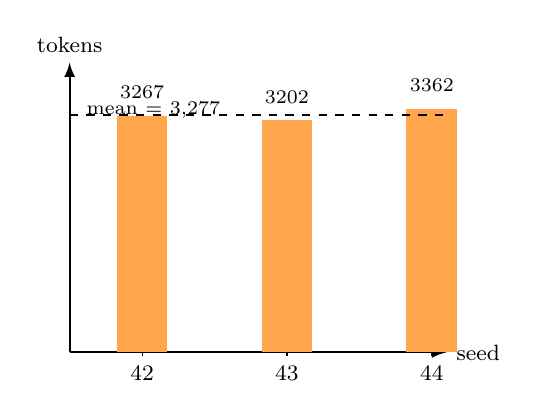
\begin{tikzpicture}[scale=0.92]
\draw[thick,-latex] (0,0) -- (5.2,0) node[right,font=\footnotesize]{seed};
\draw[thick,-latex] (0,0) -- (0,4.0) node[above,font=\footnotesize]{tokens};
\foreach \x/\name/\v in {1/42/3267, 3/43/3202, 5/44/3362}{
  \draw (\x,0.05) -- (\x,-0.05) node[below,font=\footnotesize]{\name};
  \fill[orange!70] (\x-0.35,0) rectangle (\x+0.35,\v/1000);
  \node[above,font=\scriptsize] at (\x,\v/1000+0.1){\v};
}
\draw[dashed] (0,3.277) -- (5.2,3.277);
\node[anchor=west,font=\scriptsize] at (0.1,3.34){mean = 3{,}277};
\end{tikzpicture}
\caption{Estimated tokens per run (tiktoken cl100k\_base, prompt overhead 1{,}200): 3{,}267 / 3{,}202 / 3{,}362.}
\label{fig:tokens}
\end{figure}

\subsection{Analysis}
The dominant pattern is that a careful no-rail agent already produces mostly grounded output on this structured planning task: citations are drawn from the verified pool and verify online, and numbers are either cited or are self-declared plan parameters. The single NFR hit (``7 dimensions'' in seed42) illustrates the metric's sensitivity: an uncited factual number is flagged even when the surrounding document is otherwise clean. This is exactly the class of defect the F03 numeric contract is designed to catch, and its presence in the control arm at $0.51\% \pm 0.88\%$ gives the rail arms a small but real headroom. The zero UCR reflects the task type: proposals and plans are prospective documents, so no execution claims occur; UCR will become informative in the writing-arm tasks that produce result sections.

\section{Discussion and Limitations}
\label{sec:discussion}

\textbf{Implications.} The E1 baseline shows that fabrication on a structured planning task is already low even without rails, primarily because the reference pool is small, verified, and known to the agent. This implies the strongest test for the rail hypothesis lies in more open tasks (free-form writing with unconstrained citation pools) and weaker models, where fabrication headroom is larger---consistent with our planned H3 direction.

\textbf{Limitations.} (i) Single task and single model: one representative planning task and deepseek-v4-flash only; generalization is untested. (ii) Small $n$: three seeds give a baseline anchor, not a significance test; the full comparison requires the planned paired design. (iii) NFR annotation involves a judgment call on which numbers are ``claims''; we document the rule (skip structural tokens, cite-or-design otherwise) and ship the classifier for reproducibility. (iv) Token counts are estimates from \texttt{tiktoken}, not metered API billing. (v) No LaTeX toolchain was available in the environment, so the paper compiles only on a host with TeX installed; the source is self-contained (TikZ figures, no external image files). These limits are scoped to this pre-experiment and do not weaken the planned full comparison.

\section{Conclusion}
\label{sec:conclusion}

We presented the first controlled step toward measuring the causal effect of process-level validation rails on LLM research-agent fabrication. Formalizing CFR/NFR/UCR as auditable metrics and instrumenting the unmodified no-rail pipeline, we measured a baseline of CFR $0.0\% \pm 0.0\%$, NFR $0.51\% \pm 0.88\%$, UCR $0.0\%$, completion $1.0$, one iteration, and $3{,}277 \pm 80.5$ tokens on one representative planning task over three seeds. These numbers, drawn verbatim from \texttt{experiments/results.json}, anchor the upcoming prompt-only and full-rail comparison and its cost-quality trade-off analysis. Future work runs the registered ablation and scaling experiments and extends the measurement to open-writing tasks where fabrication headroom is larger.

\bibliographystyle{plainnat}
\bibliography{references}

\end{document}
